%%
%% 研究報告用スイッチ
%% [techrep]
%%
%% 欧文表記無しのスイッチ(etitle,jkeyword,eabstract,ekeywordは任意)
%% [noauthor]
%%

\documentclass[submit,techrep]{ipsj}
%\documentclass[submit,techrep,noauthor]{ipsj}



\usepackage[dvipdfmx]{graphicx}
\usepackage{latexsym}

\def\Underline{\setbox0\hbox\bgroup\let\\\endUnderline}
\def\endUnderline{\vphantom{y}\egroup\smash{\underline{\box0}}\\}
\def\|{\verb|}

\setcounter{巻数}{53}%vol53=2012
\setcounter{号数}{10}
\setcounter{page}{1}


\begin{document}


\title{データベース及び演習\\
(2023年6月12日)}

\etitle{Database and Exercises \\ (version 2012/10/12)}

\affiliate{IPSJ}{情報処理学会\\
IPSJ, Chiyoda, Tokyo 101--0062, Japan}


\paffiliate{JU}{情報処理大学\\
Johoshori Uniersity}

\author{水谷祐生}{Yusei Mizutani}{IPSJ}[joho.taro@ipsj.or.jp]

\begin{abstract}
本稿は,情報処理学会論文誌ジャーナルに投稿する原稿を執筆する際,および論
文採択後に最終原稿を準備する際の注意点等をまとめたものである.大きく分け
ると,論文投稿の流れと,\LaTeX と専用のスタイルファイルを用いた場合の論
文フォーマットに関する指針,および論文の内容に関してするべきこと,するべ
きでないことをまとめたべからずチェックリストからなる.本稿自体も \LaTeX 
と専用のスタイルファイルを用いて執筆されているため,論文執筆の際に参考に
なれば幸いである.
\end{abstract}

%
%\begin{jkeyword}
%情報処理学会論文誌ジャーナル,\LaTeX,スタイルファイル,べからず集
%\end{jkeyword}
%
%\begin{eabstract}
%This document is a guide to prepare a draft for submitting to IPSJ
%Journal, and the final camera-ready manuscript of a paper to appear in
%IPSJ Journal, using {\LaTeX} and special style files.  Since this
%document itself is produced with the style files, it will help you to
%refer its source file which is distributed with the style files.
%\end{eabstract}
%
%\begin{ekeyword}
%IPSJ Journal, \LaTeX, style files, ``Dos and Dont's'' list
%\end{ekeyword}

\maketitle

%1
\section{機能概要}

教科書9章、10章に記されているサンプルコードにはユーザーからメールアドレス、パスワード、出身地、生年月日を受け付け、メールを用いて認証を行う会員登録機能と、会員登録を行なった後に専用ページに遷移するためのログイン機能、認証を行なった後、専用ページから退出するログアウト機能、認証されたユーザーを一覧することのできる管理者機能が実装されている.

また、全体の操作の流れは、ログイン画面から新規登録画面に遷移し、新規登録画面でメールアドレス、パスワード、出身地、生年月日を受け付ける.  その後、入力したメールアドレスで登録確認を行うとログイン者専用画面に遷移する流れとなっている.

\section{利用技術}
\subsection{PHP}
PHPとは「ピー・エイチ・ピー」と読み、Personal Home Pageがその由来である.

主に、Webで利用されるHTML形式のようなハイパーテキストを閲覧者の操作によって動的な画面を作ることを得意としている. 

PHPの特徴として誰でも無償で利用できるオープンソースのサーバサイド・スクリプト言語であることが挙げられる.さらに、無償で利用できるからと言ってメンテナンスがされていないなどはなく、マニュアル、バグ修正なども十分に行われているため、安心して利用できる. 

また、多様なDB、ライブラリへの対応、デバッグのしやすさ、その習得のしやすさなどからプログラミング言語を初めて学ぶ人たちにも扱いやすい言語となっている.

\subsection{MariaDB/MySQL}
MySQLとはオープンソースソフトウェアのRDBMD(relational database management system)であり、現在はOracle社が管理している.

一方、MariaDBとは、MySQLから派生したRDBMDであり、MySQLのソースコードをベースにして、新機能追加やソースコードの改善が組み込まれている.

両者共に互換性があり、同じSQL文を用いてデータベース操作を行なっているが、もちろん違いもある.

両者の違いとして、無償で全ての機能が使えるかどうかである.MariaDBは完全なGPLライセンスでその全ての機能が使用可能である。一方で、MySQLは特別な機能は有料のライセンスに含まれるとする、デュアルライセンス方式を採用している.

\subsection{CSS}
CSSとは(Cascading Style Sheets)は、「シー・エス・エス」と読み、Webページのデザインやレイアウトを制御する言語である. 主にHTMLやXHTMLなどで作成されるウェブページにスタイルを適用したい場合に用いられている.

CSSを使用しなくとも、HTMLには\<center\>や\<font\>タグなどの装飾目的の要素や属性が存在しているため、HTMLだけでウェブページの見栄えを制御することもできなくはない.しかし、HTMLは情報構造を定義するための言語であり、見栄えの制御のために本来の役割とは違った使い方をすると、 文書の情報構造がでたらめになってまうため、スタイリングにHTMLを用いるべきではないとされている.

そこで HTMLでは文書構造のみを定義して、 スタイルについてはCSSow用いたスタイリングシートで指定することが推奨されている.そうすることで他の閲覧環境に依存せず、HTMLを本来の役割で使用することが可能になった.


\subsection{Smarty}
Smartyとは、2000年代前半にリリースされたスクリプト言語であるPHPのテンプレートエンジンである.

テンプレートエンジンとは「機能を記述する内容(PHP)」と「画面の表示内容(HTML&CSSなど)」を分けて管理できるツールである.

単純なページや数ページ程度ではテンプレートエンジンの恩恵を感じることができないが、PCとスマートフォンで別々のレイアウトを用意したい時や、膨大なページ数を用意する場合、その便利さを感じることができる.

従来は開発の際、HTMLの中にPHPを埋め込む手法を取っていた.しかし、PHPとHTMLが混在したファイルは、2つのルールが一緒に書かれているので読み取りにくい点が難点であった.両方のプログラミング言語が混在して1つのファイルに書かれている場合、修正にはページ数が多いほど膨大な時間がかかり、保守やメンテナンスがしづらいといった問題があった.

そこで、Smatryを用いることで、機能と表示内容の分離、つまりHTMLとPHPを別のファイルで記述することができる.こうすることで、プログラマーとデザイン担当の作業ファイルを完全に分割することができるため、開発を効率的に行うことが可能になった.

\subsection{HTTP}
HTTP(HTTP: HyperText Transfer Protocol) とは、Web情報をやりとりするプロトコルの一種であり、ホームページやブログを閲覧する際、HTTPを用いてサーバとクライアント間でやり取りが行われている.

特徴として、動作がとてもシンプルであることが挙げられる.情報のやり取りは常に、クライアントが要求を出し、サーバが応答を返します。HTTPは1リクエスト1レスポンスを返すルールがあるため、どちらかが多くなることはあり得ない.また、あるリクエストに対するレスポンスは必ず同じものになる特徴がある.

このように、HTTPは完結で分かりやすい特性を持つことから、WebサーバとWebブラウザ間のやり取り以外に、スマホやアプリからのサーバ機能呼び出しや、サーバ間のサービス呼び出しなどに幅広く使われている.

\subsection{SMTP/IMAP/POP}
SMTPとはシンプル・メール・トランスファー・プロトコルと読み、Simple Mail Transfer Protocolがその由来である.主に、インターネットなどのTCP / IPネットワークで用いられており、メールを送信するための通信プロトコルの一つである.

一方でPOPとはポスト・オフィス・プロトコルと読み、Post Office Protocolがその由来である.こちらもSMTP同様にインターネットなどのTCP / IPネットワークで用いられているプロトコルであるが、SMTPと異なり、メールを受信するための通信プロトコルである.

\begin{figure}[htbp]
  \centering
 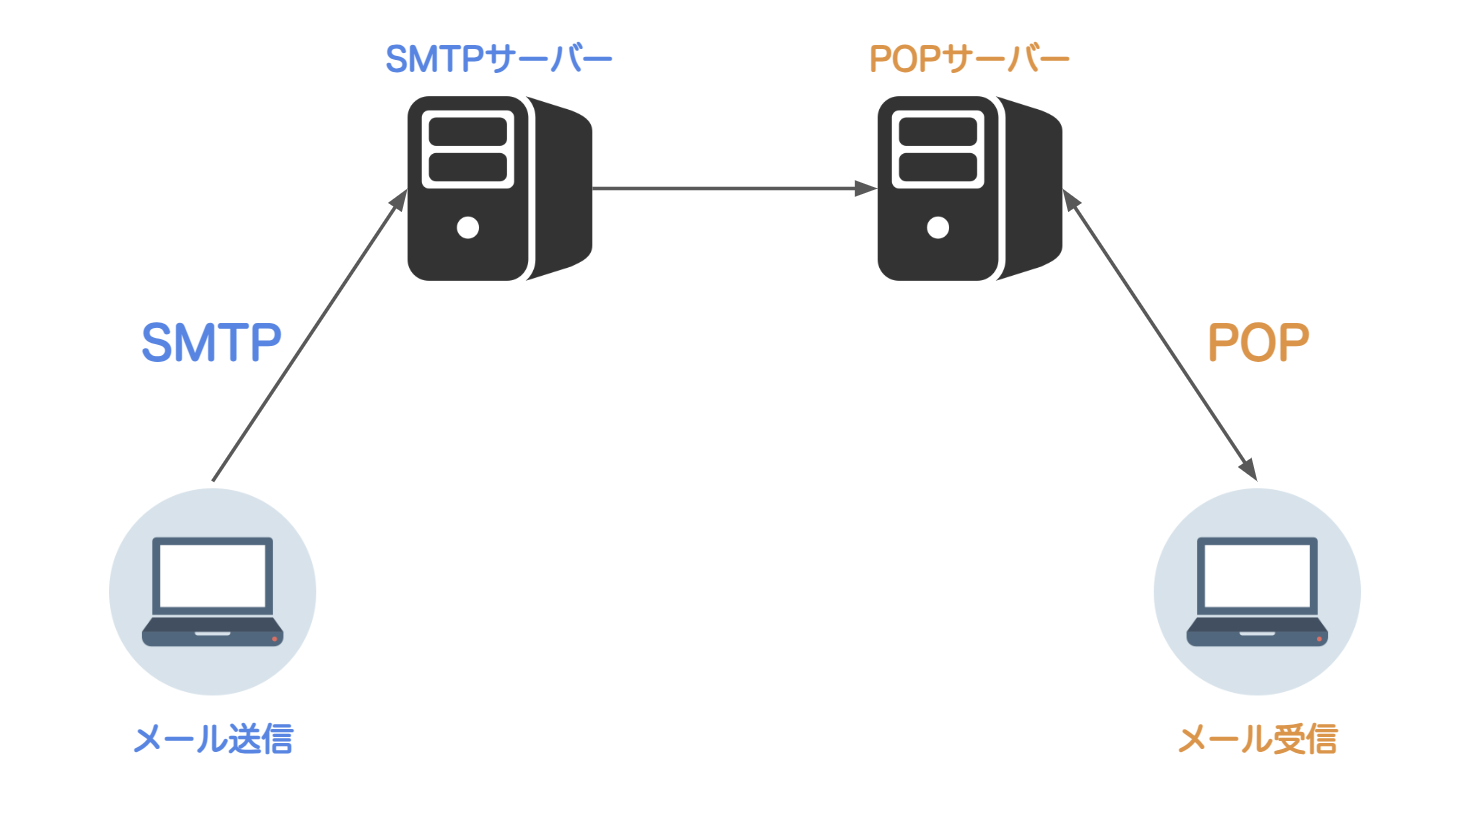
\includegraphics[width=8cm]{./images/mail.jpg}
  \caption{メール送受信の図}
  \label{fig:sample}
\end{figure}



メール送受信の仕組みとしては、上記の図のようになっており、

\begin{enumerate}
  \item SMTPでメールをサーバーに送信する
  \item SMTPサーバーからPOPサーバーに受信したメールの内容を送信する
  \item  POPサーバーから受け取る側のPCにメールの内容を送信する
  \end{enumerate}
といった流れになっている.


\section{システム設計}
\subsection{システム概要}
今回の課題で用いたサンプルコードは,必要な場合に応じてクラスを分け,それぞれのクラスの名前に対して見合ったメソッド、変数を追加している.また、作成したしたクラスを継承し、別のファイルでもクラス内のメソッドを使用できるようにしている.そうすることで、一つのファイルに処理を何百行と書く必要がなくなり、システムの保守・管理・運用を容易に行うことが可能になる.

また、今回の会員登録時に用いた入力フォームではパスワードの長さの入力チェック、つまりバリテーションを行うために、PEAEライブラリに実装しているQuickForm2を用いて、それをSmartyと連携させることで実装している.

会員専用画面である、登録後にユーザー一覧画面を表示する際は、ユーザ一覧のデータを見やすいように分割して表示するためにPagerを用いて実装している.


\subsection{画面遷移}
\subsubsection{一般会員}
\begin{figure}[htbp]
  \centering
 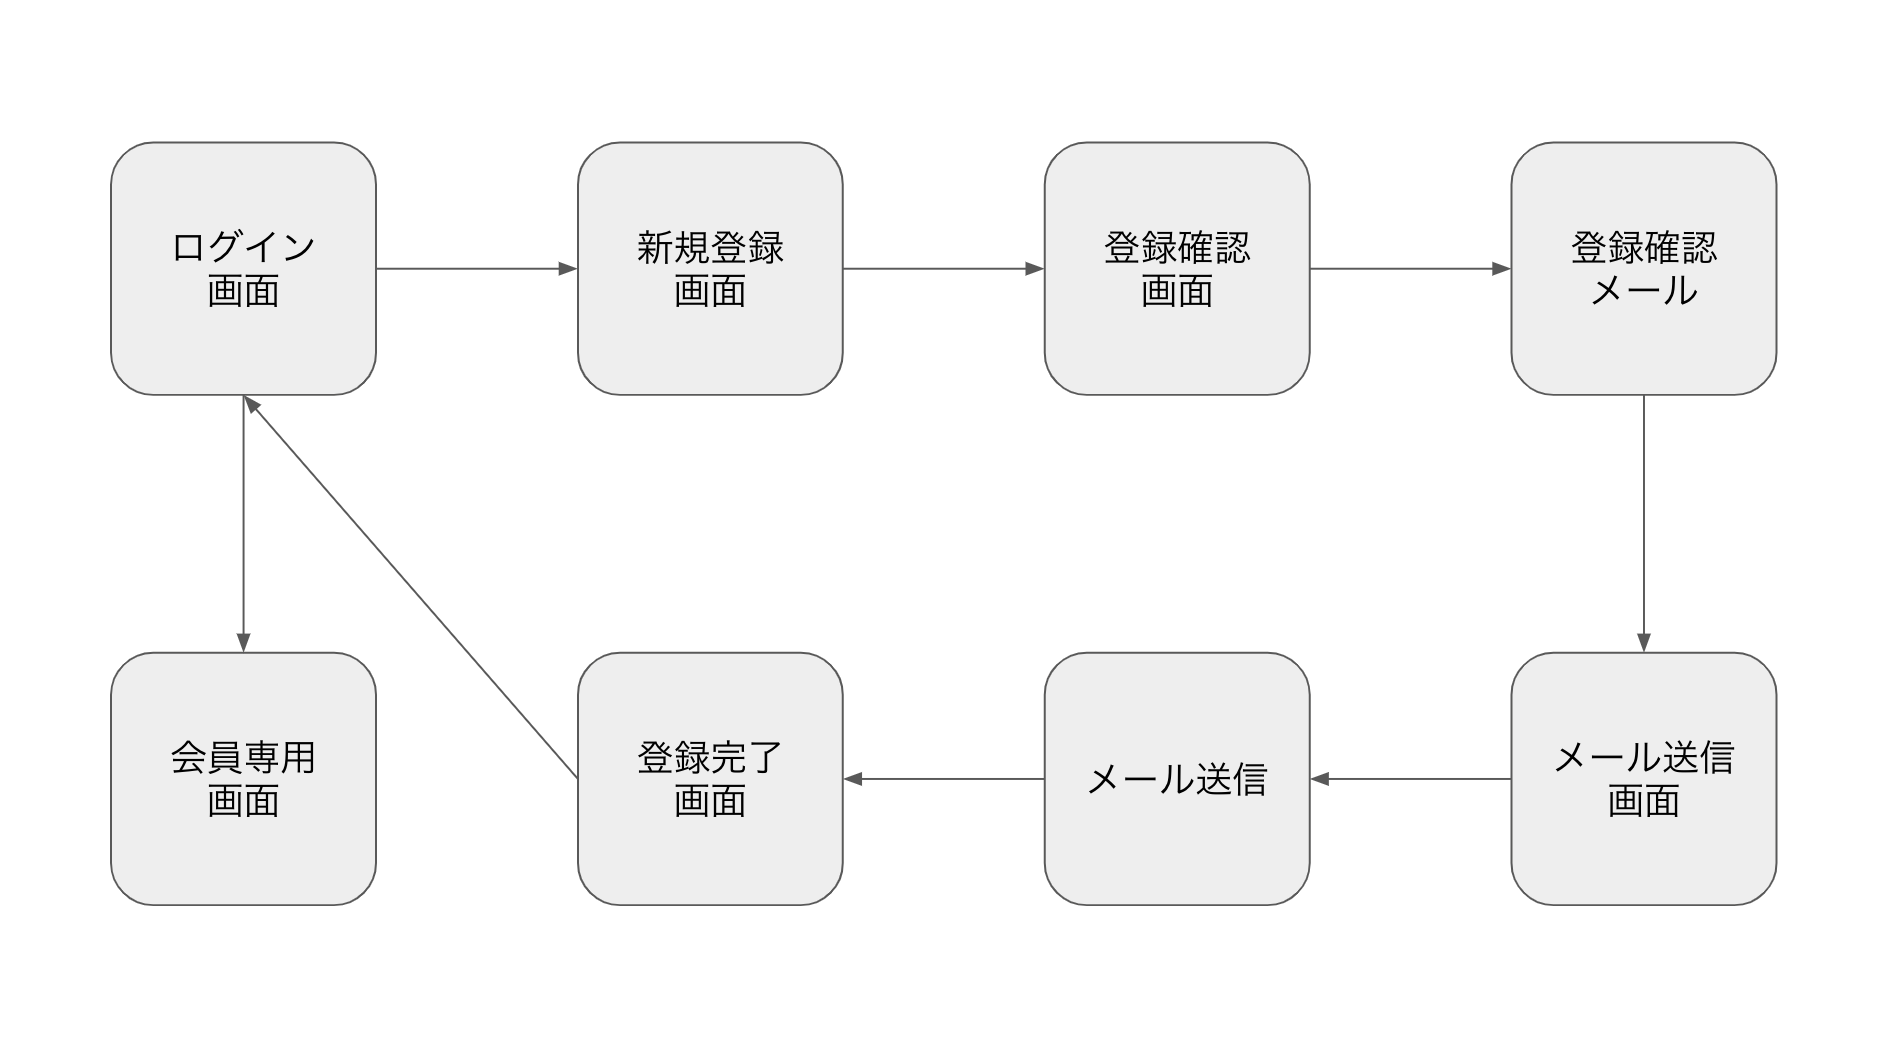
\includegraphics[width=8cm]{./images/screen_transition.jpg}
  \caption{サンプルプログラムの画面遷移の図}
  \label{fig:sample}
\end{figure}

図2は今回のサンプルプログラムにおける画面遷移を表したものであり、以下にその詳細を記す.

\begin{enumerate}
  \item ログインを行い、ログイン者専用のページに遷移する
  \item 1で新規登録をしていない場合は、新規登録画面を押して、新規登録画面に遷移する
  \item  新規登録画面に必要な項目を入力する
  \item  登録ボタンを押すと、入力内容の確認画面に遷移する
  \item  入力した内容に間違いがなかったら、登録確認用のメールを入力されたメールアドレスに送信する
  \item メールの内容を確認し、本登録が完了できたら登録完了画面に遷移し、新規登録処理を完了する
  \item  その後、ログイン画面に再度遷移する
  \item ログイン画面で、新規登録画面で入力したメールアドレスとパスワードを再度入力することで、ログイン者専用のページに遷移する
  \end{enumerate}
といった流れになっている.

\subsubsection{管理者}
\begin{figure}[htbp]
  \centering
 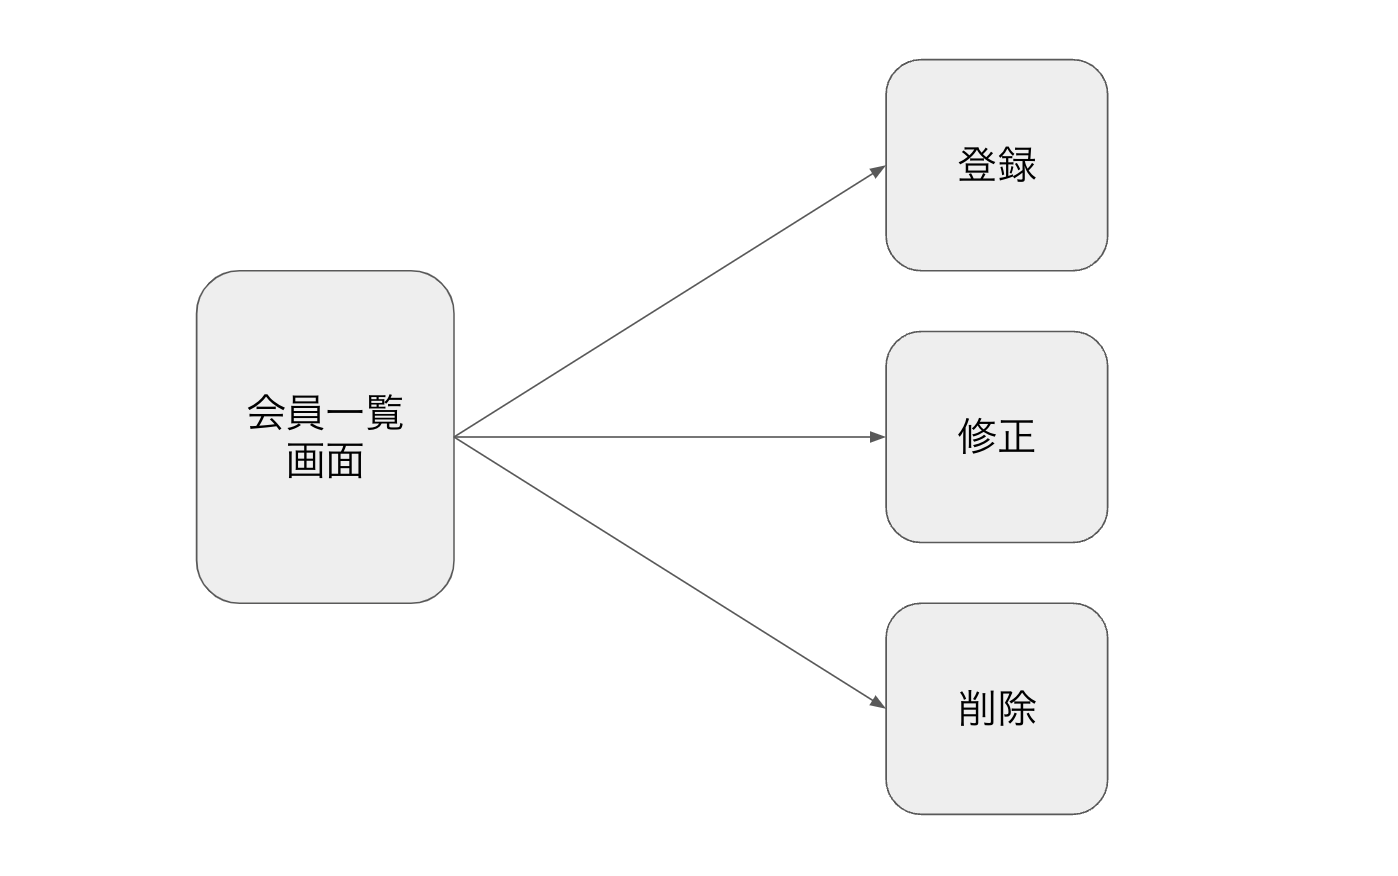
\includegraphics[width=8cm]{./images/manager_screen.jpg}
  \caption{管理者から見た画面遷移の図}
  \label{fig:sample}
\end{figure}

図3は今回のサンプルプログラムにおける管理者が行える操作を表したものであり、以下にその詳細を記す.

\begin{enumerate}
  \item 管理者専用の画面の新規登録ボタンを押すと図2の新規登録画面に遷移する
  \item 管理者専用画面の中のの会員一覧の更新ボタンを押すと、登録された会員情報の内容を修正することができる更新画面へ遷移する
  \item  管理者専用の画面の中の会員一覧に存在する削除ボタンを押すことで、登録された会員情報を削除することができる、削除確認画面に遷移する
  \end{enumerate}
といった流れになっている.

\subsection{データベース設計}
今回作成したサービスでは三つのテーブルが存在する.
一つ目は、日本の都道府県を閲覧する際に使用されるkenテーブル、二つ目は、名前、メールアドレス、パスワードなど会員情報を管理するためのmemberテーブル、三つ目はメールを用いて本登録を行っていないユーザーを仮登録として保持しておくためのprememberテーブル、これら三つのデータをMariaDB/MySQLを通して行うことでシステムを動かしている.

以下に、それぞれのテーブルについて記述していく.

\subsubsection{kenテーブル}
\begin{verbatim}
CREATE TABLE ken (
    id      SMALLINT,
    ken     VARCHAR(10),
    PRIMARY KEY (id)
);
\end{verbatim}
上のSQL文は都道府県のデータを格納するために定義されたテーブルである.

フィールドについて説明すると、idとはカラムを識別するため主キー、kenは都道府県の名前をを格納している.

\subsubsection{memberテーブル}
\begin{verbatim}
CREATE TABLE member (
    id          
    MEDIUMINT UNSIGNED NOT NULL AUTO_INCREMENT,
    username   	VARCHAR(50),
    password   	VARCHAR(128),
    last_name  	VARCHAR(50),
    first_name 	VARCHAR(50),
    birthday   	CHAR(8),
    ken         SMALLINT,
    reg_date   	DATETIME,
    cancel      DATETIME,
    PRIMARY KEY (id)
);
\end{verbatim}
上のSQL文は本登録されたユーザーのデータを格納するために定義されたテーブルである.

以下、それぞれのフィールドについて説明する

\begin{enumerate}
  \item idとはカラムを識別するため主キー、またUNSIGNED NOT NULLAUTO\_INCREMENTとは、カラムを追加される時に自動で順番にidフィールドに数字を格納するという意味である.ただし、0は受け付けない.
  \item usernameフィールドは文字列で定義されていて、カッコ内にある50とは、50バイト分の文字列まで格納できるという意味である.
 \item usernameフィールドは文字列で定義されていて、カッコ内にある50とは、50バイト分の文字列まで格納できるという意味である.
  \item passwordフィールドは文字列で定義されていて、カッコ内にある128とは、128バイト分の文字列まで格納できるという意味である.
   \item last\_nameフィールドは文字列で定義されていて、カッコ内にある50とは、50バイト分の文字列まで格納できるという意味である.
    \item first\_nameフィールドは文字列で定義されていて、カッコ内にある50とは、50バイト分の文字列まで格納できるという意味である.また、出身地の情報は都道府県を直接入れているわけではなく、kenテーブルで定義されているidを参照して管理している.こうすることでデータ量の多い都道府県の文字列よりもデータ量の少ない数値で管理できるためサーバーの負荷を軽減することができる.

  \item kenフィールドは数値で定義されていて、SMALLINTとは、-32,767 から 32,767 までの小さい整数を格納することができる意味である.
 \item reg\_dateフィールドはDARETIME型で定義されていて、YYYY-MM-DD形式で格納されている
 \item cancelフィールドはDARETIME型で定義されていて、YYYY-MM-DD形式で格納されている  \end{enumerate}

\subsubsection{prememberテーブル}
\begin{verbatim}
CREATE TABLE premember (
    id          
    MEDIUMINT UNSIGNED NOT NULL AUTO_INCREMENT,
    username   	VARCHAR(50),
    password   	VARCHAR(128),
    last_name  	VARCHAR(50),
    first_name 	VARCHAR(50),
    birthday   	CHAR(8),
    ken         SMALLINT,
    link_pass  	VARCHAR(128),
    reg_date   	DATETIME,
    PRIMARY KEY (id)
);
\end{verbatim}
上のSQL文は仮登録されたユーザーのデータを格納するために定義されたテーブルである.

基本的なフィールドはmemberテーブルとあまり差異はないが、一部異なる部分もある.link\_passフィールドである.このフィールドは本登録テーブルと仮登録テーブルの情報を結びつけるためのフィールドである.

%2.3
\subsection{システム詳細}



\begin{table}[h]
 \caption{各処理における分岐の表}
 \label{table:SpeedOfLight}
 \centering
  \begin{tabular}{lllll}
   \hline
   type & action & ボタン & 処理 & 表示画面 \\
   \hline \hline
   無し &&& 認証 & 会員画面TOP \\
   無し &&& 未認証 & ログイン画面 \\
   authenticate & - & - & 認証処理OK & 会員画面TOP \\
   authenticate & - & - & 認証処理NG & ログイン画面 \\
   regist & form & - & - & 入力画面 \\
   regist & confirm & - & 入力チェックOK & 確認画面 \\
   regist & confirm & - & 入力チェックNG & 入力画面 \\
   regist & complete & 戻る & - & 入力画面 \\
   regist & complete & 登録 & INSERT & 完了画面 \\
   modify & form & - & - & 入力画面 \\
   modify & confirm & - & 入力チェックOK & 確認画面 \\
   modify & confirm & - & 入力チェックNG & 入力画面 \\
   modify & complete & 戻る & - & 入力画面 \\
   modify & complete & 登録 & UPDATE & 完了画面 \\
   delete & confirm & - & - & 入力画面 \\
   delete & complete & - & DELETE & 完了画面 \\
   modify & - & - & ログアウト処理 & ログイン画面 \\
   \hline
  \end{tabular}
\end{table}

表2は,typeとactionの値によって,振り分けられるときの条件を表したものである.次の画面へ遷移されるときリンクをクリックして画面を表示させるときか、送信ボタンを押して画面を表示させるときのいずれかである. 送信ボタンを押して、画面遷移する場合は、HTTPのGETメソッドにより、パラメーターをURLに載せて、サーバに送信している.送信ボタンを押して画面遷移する場合は、HTTP の POST メソッドを用いて、ユーザーからは確認できないよう安全に値が送信される.

ここで、GETメソッドとPOSTメソッドの違いについて説明する.

GETメソッドはURLにパラメータを含めることで、サーバーに情報を送るHTTPリクエストの一つである.主に、あるページを取得するためにサーバーにリクエストを送る際にこのメソッドが用いられる.

POSTメソッドとはパラメータをリクエストヘッダーに含めることで、サーバーとデータのやり取りを行うHTTPリクエストの一つである.GETメソッドと明確に異なる点として、サーバーに送った情報がユーザーには見ることができない点が挙げられる.この特徴によりPOSTメソッドは、主にデータを追加する際、今回のサンプルプログラムだとユーザーの仮登録、本登録をする際、個人情報などといった第三者に見られてはいけない情報を送信する際に用いられる.

メソッドの決め方としては、\$this-\>type の値でメソッドが決まり、メソッドの内部では\$this-\>action の値で処理を振り分けていく.また,送信ボタンが二つある画面では,ボタンの名称を振り分けに利用している.

\subsection{変数設計}

\subsection{各画面設計}
各画面はQuickForm2、Smarty により、PHPファイルをもとに自動生成されている.

画面描写に必要なファイルはsmatryディレクトリのtemplatesディレクトリ内にある.tplファイルである.これらのファイルを読み込むことで、画面を描写することができる.

\subsubsection{ログイン画面}
ログイン画面の描写には、login.tplを用いている

index.phpの情報を参照することでセッション管理を行なっていて、ログイン済みであると認証されなかった場合は、このページに遷移するようになっている.

また、入力欄に入力した内容をブラウザ側で保持しつつ出るために、\$form.username.labelには,ユーザー名を格納し、\$form.username.htmlはユーザー名の入力欄、HTMLのコードに置き換わる.同様に、\$form.password.labelはパスワード名に、\$form.password.htmlはパスワー ド入力欄にHTMLのコードに置き換わる.

\subsubsection{仮登録表示画面}
画面の描写にはpremember.tplが用いられる.

新規登録画面から確認画面でユーザーが登録情報を確認した後に遷移する画面であり、メールを送信した旨を伝えるための画面である.

\subsubsection{会員専用画面}
画面の描写にはmember\_top.tplが用いられる.

ログインを終えた会員とindex.phpにセッションが残っている場合は子も画面に遷移する.

\subsubsection{管理者専用画面}
画面の描写にはsystem\_login.tplが用いられる.

管理者用のパスワードを入力し、認証を終えると、このページに遷移する.
会員一覧へのリンクは\$SCRIPT\_ NAME?type=list\& action=formとなり\$ SCRIPT\_ NAMEはsystem.phpに置き換わる。 クリックするとsystem.phpに対してtype=listとaction=formが送信され、会員一覧を表示する。

\section{実装}

\subsection{実装環境}
\begin{table}[h]
 \caption{用いたツール名とそのバージョンの表}
 \label{table:SpeedOfLight}
 \centering
  \begin{tabular}{ll}
   \hline
   名前 & バージョン  \\
   \hline \hline
  OS & macOS Venture バージョン 13.4 \\
  XAMPP &  7.4.28 \\
  PHP & 7.4.28 \\

   \hline
  \end{tabular}
\end{table}

今回は以上の表のような環境で動作確認を行なった.

\subsection{環境設定}
今回のサンプルプログラムを動作させるために必要なXAMPPの環境構築は以下のように行なった.

\begin{enumerate}
  \item 公式サイトからXAMPPをインストールする
  \item 設定を行い、XAMPPコントロールパネルを起動させる
  \item  WebサーバーであるApacheを起動させる
  \end{enumerate}
といった流れになっている.

次に実際に今回のシステムを動作させるためのプログラムの配置は以下の手順で行なった

\begin{enumerate}
  \item 「環境構築から実践的なシステム作成まで完全習得! PHP7+MariaDB/MySQL マスターブック」に記されているサンプルデータにアクセスする
  \item そこにあるSection77の内容を引用するために、XAMPPディレ クトリにphp\_libsを作成し、htdocsとphp\_libsに引用したサンプルプログラムをすべて移す.
データの Section77 に入っているすべてのファイルを移す。
  \item  コピペしたフォルダにあるファイルにアクセス権を付与する
  \end{enumerate}
  
  
  MySQLの初期設定は以下の手順で行なった.
\begin{enumerate}
  \item sqlフォルダを作成する
  \item サンプルプログラムのSection76、Section86からにあるSQLファイルをコピーして、sqlフォルダに格納する
  \item MySQLにアクセスし、予め、データベースやテーブル、初期ユーザーをインサートしておく
  \end{enumerate}
といった流れになっている.

今回のサンプルプログラムでは、メールを受け取って、本登録を完了する機能が実装されている.そこで、gmailのメール受け取りに関する設定が必要になっため、その手順を以下に記す.


\begin{enumerate}
  \item gmailのWebページにアクセスする
  \item 右上の歯車のアイコンをクリックする
  \item 押すと、「全ての設定を表示」という項目が表示されるためそれをクリックする
  \item 「メール転送とPOP/IMAP」をクリックする
  \item 「IMAPアクセス」のステータスを「IMAP を有効にする」に変更する
  \end{enumerate}
  
   \begin{figure}[htbp]
  \centering
 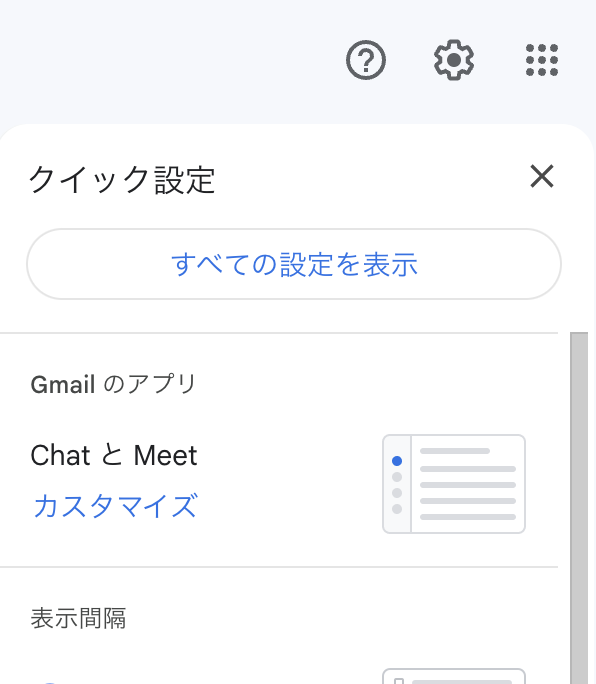
\includegraphics[width=8cm]{./images/all_setting.jpg}
  \caption{全ての設定を表示ボタンが表示されている画面の図}
  \label{fig:sample}
\end{figure}
  
  \begin{figure}[htbp]
  \centering
 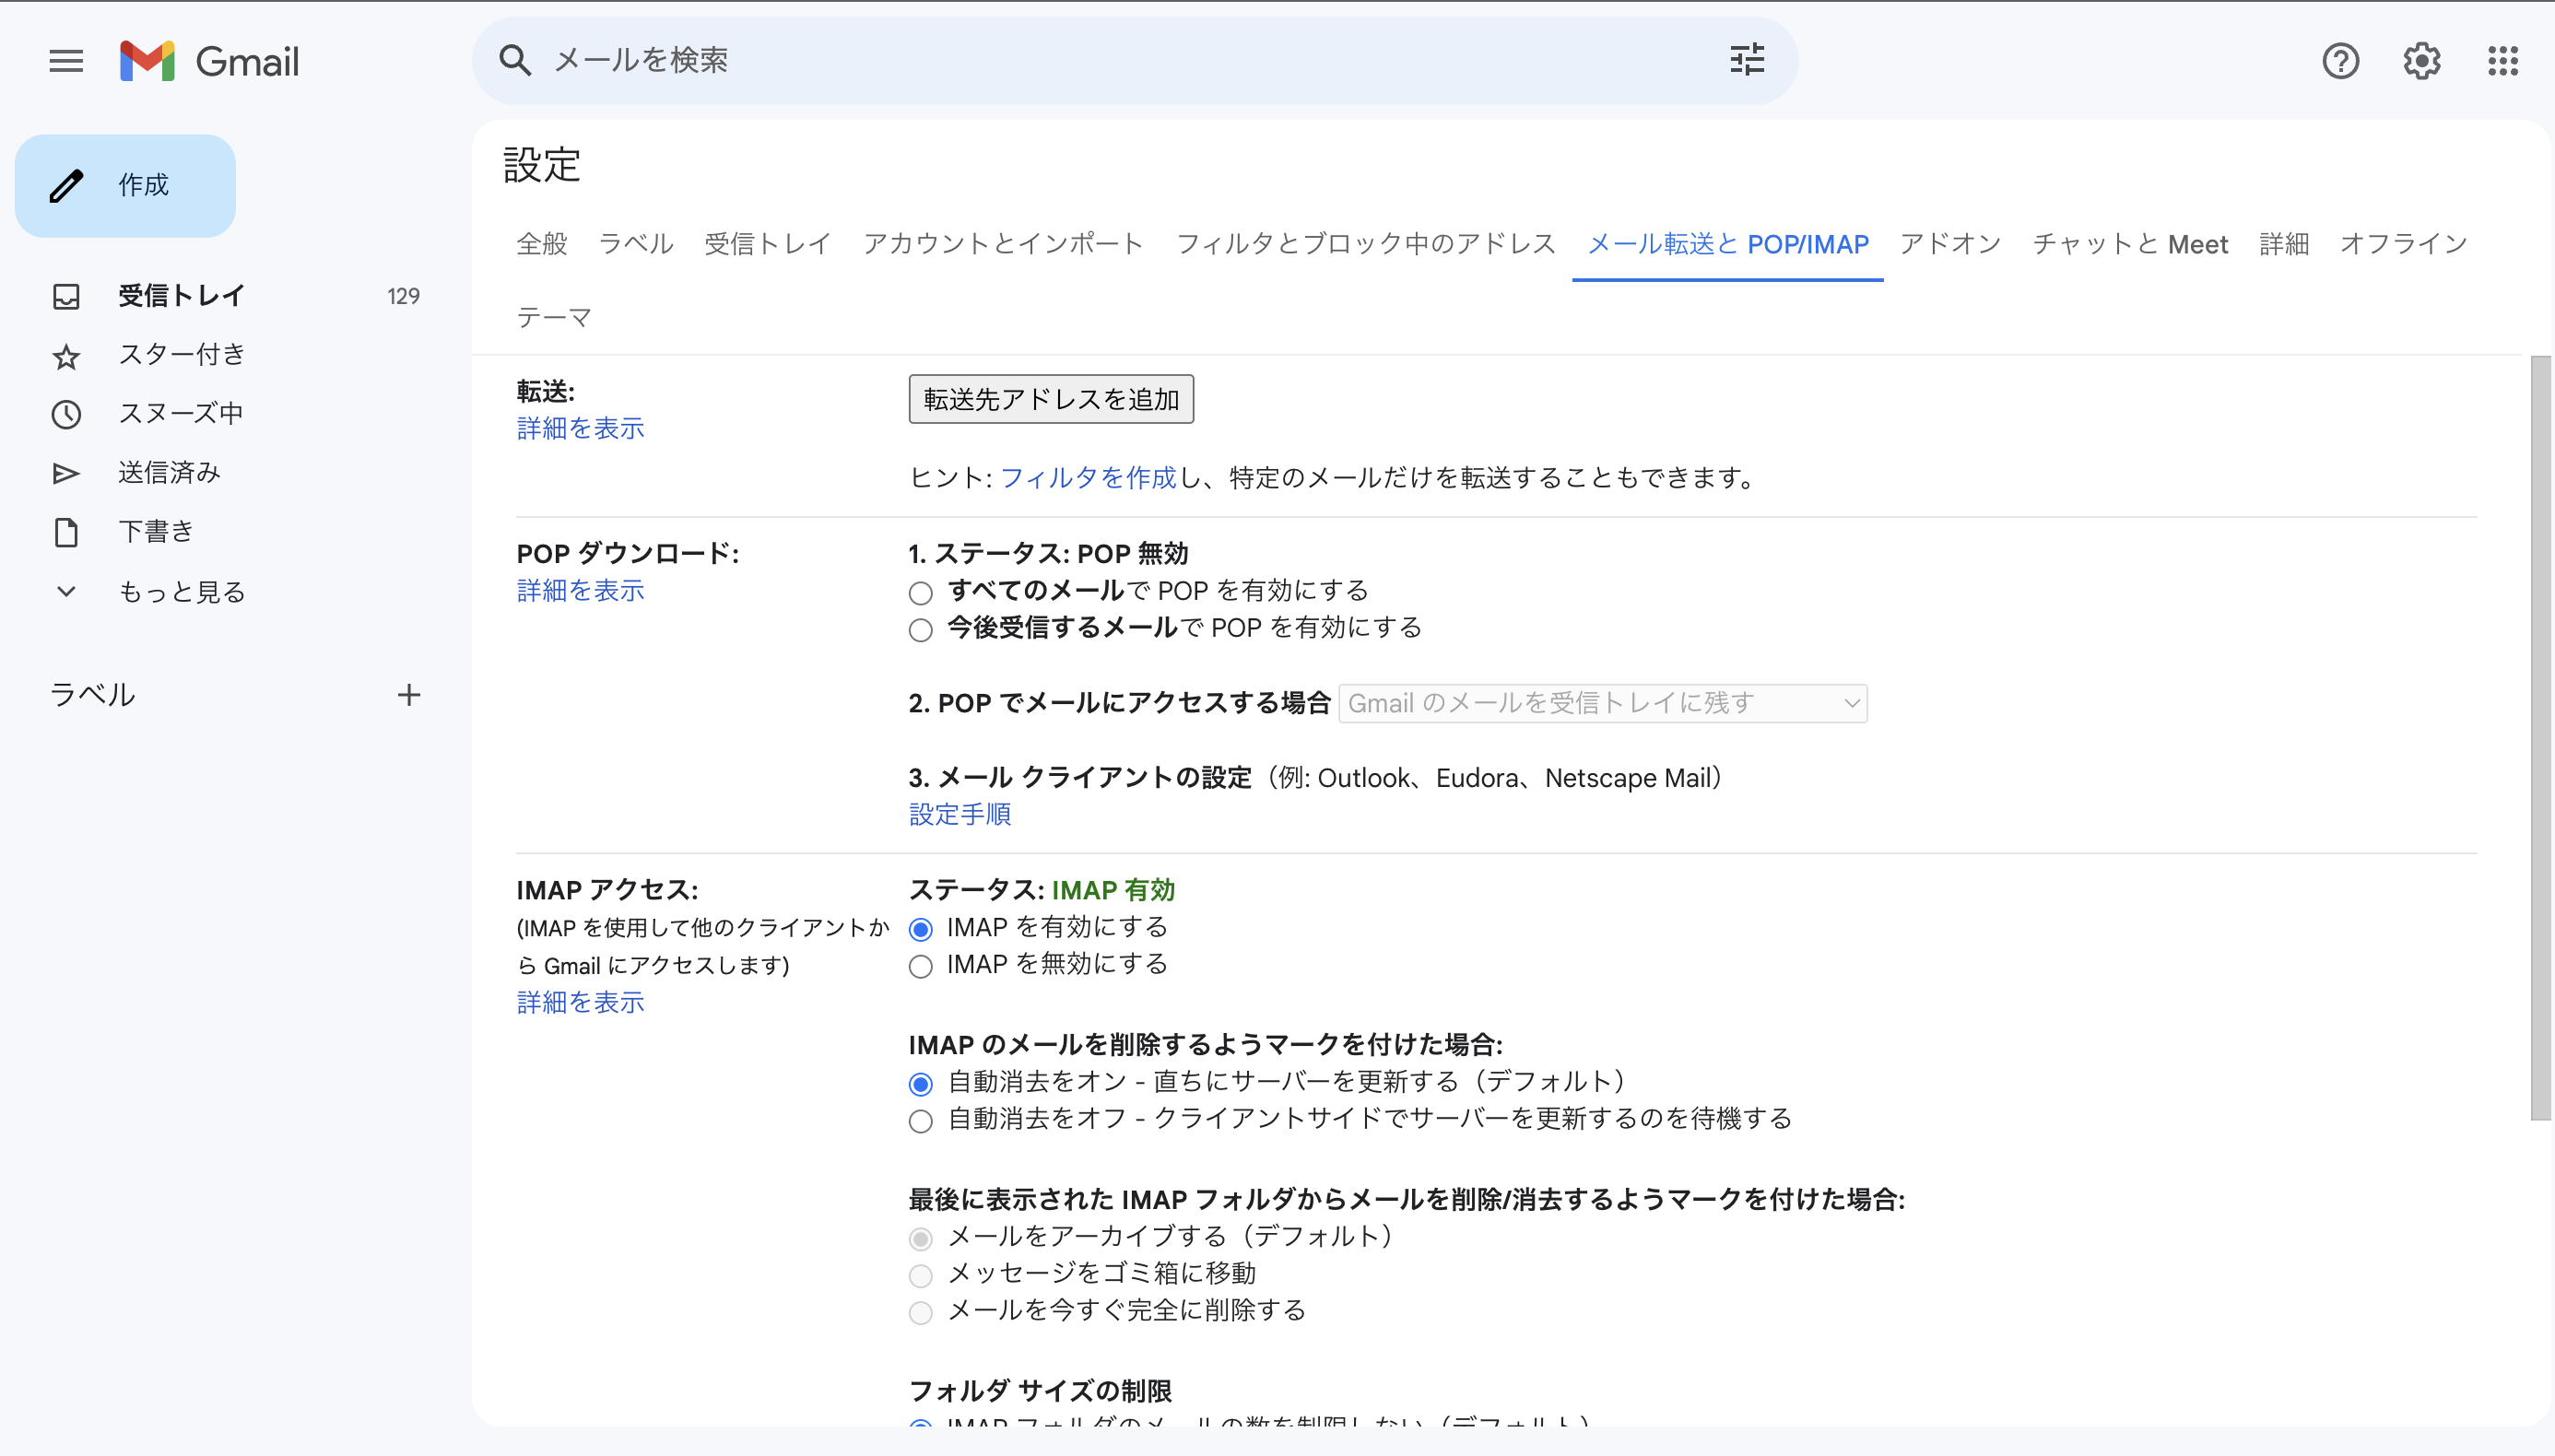
\includegraphics[width=8cm]{./images/pop_imap.jpg}
  \caption{IMAPを有効にした時の画面図}
  \label{fig:sample}
\end{figure}

以上の手順を踏むと、Gmailのコンソール画面のうちIMAPアクセス」のステータスを「IMAP を有効にする」に変更でき、IMAPサーバーからPOPサーバーにメールの内容を送信できるようになる.

また、本来Smatryを利用する際はインストールするまでに必要な手順を踏む必要があるが、サンプルプログラムを引用することでその必要は無くなったため、説明は省略することにする.

\subsection{動作検証}
画面遷移の説明の際に用いた図2の手順を踏んで行なった.
まずは一般会員に関する動作検証を行なった.
\begin{enumerate}
  \item ログイン画面では自分の入力した内容がフォームにもそのまま反映されるかを検証した
  \item 新規登録画面ではログイン画面同様、フォームにもそのまま反映されるかに加えデータベースに格納されている都道府県情報が選択できているかを検証した
  \item 登録確認画面ではユーザーが新規登録画面で入力した値がprememberテーブルに格納され、表示できているか検証
  \item メール確認後、本登録が完了した旨を伝える画面が表示されるかを検証
  \item 再びログイン画面に遷移した時、新規登録で登録したメールアドレス、パスワードでログインを行えるか検証
   \item 会員専用画面で、登録内容の修正、削除、ログアウトが行えるか検証
  \item 「IMAPアクセス」のステータスを「IMAP を有効にする」に変更する
   \item 「メール転送とPOP/IMAP」をクリックする
  \item 「IMAPアクセス」のステータスを「IMAP を有効にする」に変更する
  \end{enumerate}
  
 次には管理者に関する動作検証を行なった.
\begin{enumerate}
  \item ログイン画面で管理者用のパスワードを入力することで管理者用のページに遷移することができるかを検証した
  \item 管理者ページから会員一覧ページに遷移できるか検証
  \item 会員一覧ページでは、会員情報を全て閲覧できるようになっているか、またそれを削除、修正することができるかを検証
  \item メール確認後、本登録が完了した旨を伝える画面が表示されるかを検証
  \item 再びログイン画面に遷移した時、新規登録で登録したメールアドレス、パスワードでログインを行えるか検証
  \end{enumerate}
  
  以上のように一般会員、管理者の動作検証を行ったところ、画面遷移や表示内容、処理について全く不具合が確認できなかったため、システムは正常に動作していると判断した.
  
\section{まとめ}
今回のサンプルプログラムではPHPとMySQLを連携させて作る簡単な会員登録アプリを作成した.普段、個人またはチームでアプリ開発に取り組む際は、便利なライブラリに頼ったり、Firebaseに認証機能を任せていたりしているためメール認証で使われるSMTPサーバー、POPサーバーについて深く知ることができたことはとても良い経験になった.

アプリ全体を通して、いつデータベースにアクセスして削除、追加、閲覧を行ったらよいのか、また、セッションとクッキーの管理、バリテーション、メール送信機能が実装されているため、基本的なアプリの流れを知ることができるアプリであった.

また、今回のアプリは新規登録を行なってログインをして、ログイン者専用ページを表示するといったとてもシンプルなものであったが、今後、会員専用ページに機能を拡張していくことでより面白いアプリにすることができる基盤となるアプリであるとも考えた.



%% 以下は無視されます

\begin{biography}
\profile{m}{情報 太郎}{1970年生.1992年情報処理大学理学部情報科学科卒.
1994年同大大学院修士課程了.同年情報処理学会入社.オンライン出版の研究
に従事.電子情報通信学会,IEEE,ACM 各会員}
%
\profile{n}{処理 花子}{1960年生.1982年情報処理大学理学部情報科学科卒.
1984年同大大学院修士課程了.1987年同博士課程了.理学博士.1987年情報処
理大学助手.1992年架空大学助教授.1997年同大教授.オンライン出版の研究
に従事.2010年情報処理記念賞受賞.電子情報通信学会,IEEE,IEEE-CS,ACM
各会員}
%
\profile{s}{学会 次郎}{1950年生.1974年架空大学大学院修士課程了.
1987年同博士課程了.工学博士.1977年架空大学助手.1992年情報処理大学助
教授.1987年同大教授.2000年から情報処理学会顧問.オンライン出版の研究
に従事.2010年情報処理記念賞受賞.情報処理学会理事.電子情報通信学会,
IEEE,IEEE-CS,ACM 各会員}
%
\end{biography}



\end{document}
